%%%%%%%%%%%%%%%%%%%%%%%%%%%%%%%%%%%%%%%%%
% Journal Article
% LaTeX Template
% Version 1.4 (15/5/16)
%
% This template has been downloaded from:
% http://www.LaTeXTemplates.com
%
% Original author:
% Frits Wenneker (http://www.howtotex.com) with extensive modifications by
% Vel (vel@LaTeXTemplates.com)
%
% License:
% CC BY-NC-SA 3.0 (http://creativecommons.org/licenses/by-nc-sa/3.0/)
%
%%%%%%%%%%%%%%%%%%%%%%%%%%%%%%%%%%%%%%%%%

%----------------------------------------------------------------------------------------
%	PACKAGES AND OTHER DOCUMENT CONFIGURATIONS
%----------------------------------------------------------------------------------------

%\documentclass{article}
%\documentclass[oneside,twocolumn]{article}
\documentclass[oneside,onecolumn]{article}

\usepackage{blindtext} % Package to generate dummy text throughout this template 
\usepackage{multicol}
\usepackage[sc]{mathpazo} % Use the Palatino font
\usepackage[T1]{fontenc} % Use 8-bit encoding that has 256 glyphs
\linespread{1.05} % Line spacing - Palatino needs more space between lines
\usepackage{microtype} % Slightly tweak font spacing for aesthetics

%\usepackage[english]{babel} % Language hyphenation and typographical rules
\usepackage[spanish]{babel}
\usepackage[hmarginratio=1:1,top=32mm,columnsep=20pt]{geometry} % Document margins
\usepackage[hang, small,labelfont=bf,up,textfont=it,up]{caption} % Custom captions under/above floats in tables or figures
\usepackage{booktabs} % Horizontal rules in tables

\usepackage{lettrine} % The lettrine is the first enlarged letter at the beginning of the text

\usepackage{listings} % Required for insertion of code

\usepackage{enumitem} % Customized lists
\setlist[itemize]{noitemsep} % Make itemize lists more compact

\usepackage{abstract} % Allows abstract customization
\renewcommand{\abstractnamefont}{\normalfont\bfseries} % Set the "Abstract" text to bold
\renewcommand{\abstracttextfont}{\normalfont\small\itshape} % Set the abstract itself to small italic text

\usepackage{titlesec} % Allows customization of titles
\renewcommand\thesection{\Roman{section}} % Roman numerals for the sections
\renewcommand\thesubsection{\roman{subsection}} % roman numerals for subsections
\titleformat{\section}[block]{\large\scshape\centering}{\thesection.}{1em}{} % Change the look of the section titles
\titleformat{\subsection}[block]{\large}{\thesubsection.}{1em}{} % Change the look of the section titles

\usepackage{fancyhdr} % Headers and footers
\pagestyle{fancy} % All pages have headers and footers
\fancyhead{} % Blank out the default header
\fancyfoot{} % Blank out the default footer
%\fancyhead[C]{Running title $\bullet$ May 2016 $\bullet$ Vol. XXI, No. 1} % Custom header text
\fancyfoot[RO,LE]{\thepage} % Custom footer text

\usepackage{titling} % Customizing the title section

\usepackage{hyperref} % For hyperlinks in the PDF

\usepackage{listings}
\usepackage{algorithm2e}
\usepackage{graphicx}
\usepackage[dvipsnames]{xcolor}
\definecolor{codegreen}{rgb}{0,0.6,0}
\definecolor{codegray}{rgb}{0.5,0.5,0.5}
\definecolor{codepurple}{rgb}{0.58,0,0.82}
\definecolor{backcolour}{rgb}{1,1,1}
\lstdefinestyle{mystyle}{
    backgroundcolor=\color{backcolour},   
    commentstyle=\color{codegreen},
    keywordstyle=\color{magenta},
    numberstyle=\tiny\color{codegray},
    stringstyle=\color{codepurple},
    basicstyle=\ttfamily\footnotesize,
    breakatwhitespace=false,         
    breaklines=true,                 
    captionpos=b,                    
    keepspaces=true,                 
    numbers=left,                    
    numbersep=5pt,                  
    showspaces=false,                
    showstringspaces=false,
    showtabs=false,                  
    tabsize=2
}
\renewcommand{\lstlistingname}{Código}% Listing -> Algorithm
\lstset{style=mystyle}

\usepackage[utf8]{inputenc} % Required for inputting international characters
\usepackage[T1]{fontenc} % Output font encoding for international characters

\usepackage{amsmath}
%----------------------------------------------------------------------------------------
%	TITLE SECTION
%----------------------------------------------------------------------------------------

\setlength{\droptitle}{-4\baselineskip} % Move the title up

\pretitle{\begin{center}\Huge\bfseries} % Article title formatting
\posttitle{\end{center}} % Article title closing formatting
\title{Algoritmo Bug2} % Article title
\author{%
\textsc{Luis Alberto Ballado Aradias} \\%\thanks{A thank you or further information} \\[1ex] % Your name
\normalsize Cinvestav Unidad Tamaulipas \\ % Your institution
\normalsize luis.ballado@cinvestav.mx % Your email address
%\and % Uncomment if 2 authors are required, duplicate these 4 lines if more
%\textsc{Jane Smith}\thanks{Corresponding author} \\[1ex] % Second author's name
%\normalsize University of Utah \\ % Second author's institution
%\normalsize \href{mailto:jane@smith.com}{jane@smith.com} % Second author's email address
}
\date{\today} % Leave empty to omit a date
\renewcommand{\maketitlehookd}{%
  \begin{abstract}
    \noindent El presente trabajo describe la implementación del algoritmo bug2, con ayuda de los módulos desarrollados anteriormente como el de odometría para un robot móvil de tipo diferencial y su implementación bajo el lenguaje NXC (Not eXactly C).\\
    El algoritmo Bug2 es un algoritmo de navegación en robótica que se utiliza para que un robot encuentre su camino hacia un destino en un ambiente desconocido, sin la necesidad de utilizar un mapa previamente construido. Este algoritmo se basa en la idea de que el robot puede seguir la pared del obstáculo que se encuentra en su camino hacia el destino.
  \end{abstract}
}

%----------------------------------------------------------------------------------------

\begin{document}

% Print the title
\maketitle

%----------------------------------------------------------------------------------------
%	ARTICLE CONTENTS
%----------------------------------------------------------------------------------------
\section{Introducción}

\lettrine[nindent=0em,lines=3]{E}l algoritmo Bug2 es un algoritmo de navegación en robótica que se utiliza para guiar a un robot hacia un destino en un ambiente desconocido sin la necesidad de tener un mapa previamente construido. Este algoritmo se basa en la idea de que el robot puede seguir la pared del obstáculo que se encuentra en su camino hacia el destino, es una mejora del algoritmo Bug1, el cual tenía la limitación de que el robot podía quedar atrapado en situaciones donde no había un camino claro hacia el destino. El algoritmo Bug2 resuelve este problema al permitir que el robot se aleje temporalmente del obstáculo para encontrar una forma de continuar hacia el destino.\\

Este algoritmo es especialmente útil en aplicaciones de robótica móvil, donde el robot debe navegar en un ambiente desconocido y no se dispone de un mapa previamente construido. Además, es una técnica simple y fácil de implementar, lo que lo hace adecuado para aplicaciones en las que se requiere una navegación autónoma en tiempo real. En esta técnica, el robot utiliza sensores para detectar obstáculos y para determinar la dirección y la distancia al destino. A partir de esta información, el algoritmo guía al robot para que siga la pared del obstáculo en su camino hacia el destino.\\

También se ha utilizado en aplicaciones de seguridad, como la vigilancia y el control de fronteras, y en aplicaciones de rescate, como la búsqueda y rescate en zonas de desastre.\\

En general, el algoritmo Bug2 es una técnica importante en el campo de la robótica móvil que ha permitido el desarrollo de robots autónomos capaces de navegar en ambientes desconocidos. Su simplicidad y facilidad de implementación lo hacen adecuado para una amplia gama de aplicaciones, y las mejoras y extensiones continuas lo mantienen relevante y valioso en la investigación y el desarrollo de robótica móvil.

\newpage
\section{Vehículos de Braitenberg}

Los vehículos de Braitenberg son robots simples y autónomos diseñados para demostrar los conceptos de comportamiento emergente y robótica comportamental. Estos robots fueron desarrollados por el neurocientífico italiano Valentino Braitenberg en la década de 1980 como un medio para explorar la relación entre los sistemas sensoriales y motores en los seres vivos y los robots.\\

Se componen de uno o varios sensores y motores que están interconectados de manera específica para generar diferentes comportamientos. Estos comportamientos pueden ser desde simples movimientos en respuesta a la estimulación sensorial hasta comportamientos más complejos, como la evasión de obstáculos o la búsqueda de fuentes de luz.\\

Los vehículos de Braitenberg han sido utilizados en la investigación y la educación en robótica debido a su simplicidad y facilidad de construcción y programación. Además, han demostrado ser una herramienta valiosa para entender cómo los sistemas simples pueden dar lugar a comportamientos complejos y emergentes, también han sido utilizados en la investigación en neurociencia para estudiar los principios de la percepción y el movimiento en los seres vivos. Esto se debe a que los vehículos de Braitenberg se asemejan a los sistemas sensoriales y motores de los animales y pueden utilizarse para investigar cómo estos sistemas interactúan y generan comportamientos complejos.\\

En general, los vehículos de Braitenberg son una herramienta valiosa en la investigación y educación en robótica y neurociencia. Su simplicidad y facilidad de construcción y programación permiten a los estudiantes y los investigadores explorar los principios fundamentales de la robótica y la biología sin necesidad de conocimientos especializados en programación o ingeniería.\\

\begin{figure}[h]
  \centering
  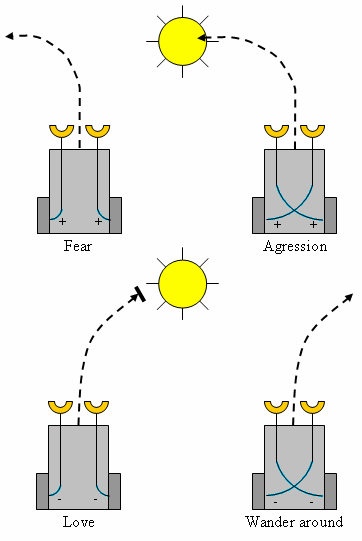
\includegraphics[scale=0.4]{graficos/braitenberg.png}
  \caption{Vehículos de Braitenberg}
\end{figure}

\newpage
\section{Algoritmo Bug2}

La relación entre el algoritmo Bug2 y los vehículos de Braitenberg radica en el hecho de que ambos utilizan principios simples para generar comportamientos complejos y emergentes. En el caso de los vehículos de Braitenberg, esto se logra mediante la interconexión de sensores y motores de manera específica. En el caso del algoritmo Bug2, esto se logra mediante el uso de un sensor y motores para permitir que el robot interactúe con su entorno de manera autónoma.

\begin{figure}[h]
  \centering
  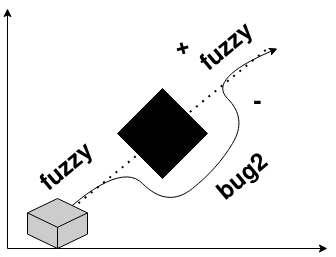
\includegraphics[scale=0.7]{graficos/bug2.png}
  \caption{Ejemplo de implementación}
\end{figure}

El algoritmo bug2 se describe a continuación

\SetKwComment{Comment}{/* }{ */}

\begin{algorithm}
  \caption{Algoritmo Bug2}\label{alg:two}
  \While{no en el objetivo}{
    seguir navegando \Comment*[r]{si aún no llegamos al objetivo}
    \If{detectamos un obstáculo}{ 
      seguir el obstáculo por su borde hasta encontrar el punto más cercano que nos regrese al control de navegacion\;
    }\Else{
      apagar\_motores\;
      llegué al objetivo\;
    }
  }
\end{algorithm}

Partiendo de la sencillez del algoritmo, lo que falta es poder identificar la región donde pueda cambiar hacia el control difuso nuevamente. Para ello seguimos haciendo uso de los valores que nuestro odometro nos brinda en todo momento.

\subsection{Cambio de control}

Una de los objetivos son los cambios de control.\\

Partiendo de la navegación, al detectar un obstáculo.

\begin{enumerate}
\item Guardar la posición cuando se detecta un obstáculo.
\item Calcular el vector x,y respecto a la distancia entre el punto donde se detectó el obstáculo y el punto final.
\item Rotar el vector x,y $90^{\circ}$
\item Efectuar la diferencia entre las lecturas del odometro con la posición donde se dectó el obstáculo.
\item Multiplicar la diferencia con los elementos del vector para obtener el vector resultante
\item Identificar el cambio de signo del resultado anterior
\end{enumerate}


\section{Implementación}

Nuestra implementación es la combinación de las practicas anteriores como odometría y el control difuso para ir del origen a un punto $x_f,y_f$.\\

Partimos de la necesidad de cambiar de controles respecto a la situación que se presenta.
\begin{itemize}
\item Control de lógica difusa: Navegar de punto $A \rightarrow B$
\item Control Boundary Following: Rodear el obstáculo
\item Cálculo para identificar si rodie el obstáculo
\end{itemize}

A continuación se describe el pseudocódigo que describe el comportamiento de la implementación

\SetKwComment{Comment}{/* }{ */}

\begin{algorithm}
  \caption{Cambio entre controles}\label{alg:two}
  Comenzar con fuzzy\_control()\;
  \While{true}{
    seguir\_con\_control\_fuzzy \Comment*[r]{si aún no llegamos al objetivo}
    \If{$a$ > 4}{ 
      \If{sensor\_frente < 30}{ 
        Apagar\_Motores \Comment*[r]{si el sensor de enfrete detecta un obstáculo}
        definir $x_0, y_0$ \Comment*[r]{guardar x,y donde encontre un obstáculo}
        goto follow\_b \Comment*[r]{cambiar al control follow\_boundary}
      }
    }\Else{
      apagar\_motores\;
      llegué al objetivo\;
    }
  }
  
\end{algorithm}

\newpage
Para el control de follow boundary se tiene

\SetKwComment{Comment}{/* }{ */}

\begin{algorithm}
  \caption{Rodear obstáculo}\label{alg:two}
  calculos\_signo = 0 \Comment*[r]{variable para detectar los cambios de signo}
  Rotar\_robot\_30Grados() \Comment*[r]{rotar robot para que el sensor de izquierda obtenga lecturas}
  \While{true}{
    \If{sensor\_izquiera < 10}{
      $error\_izquierda \gets 0$
    }\ElseIf{sensor\_izquierda < 100}{
      $error_izquierda \gets (30 - us\_izquierda)*2$
    }
    
    \If{sensor\_izquierda > 100}{ 
      error\_izquierda = -10\;
    }

    potencia\_motor\_izquierda = 50 + error\_izquierda\;
    potencia\_motor\_derecha = 50 - error\_izquierda\;

    vx = ($x_f-x_0$) \Comment*[r]{calcular vector $x_0 x_f$}
    vy = ($y_f-y_0$) \Comment*[r]{calcular vector $y_0 y_f$}

    n[0] = -vy \Comment*[r]{rotar 90 grados}
    n[1] = vx\;
    
    ODO\_$X_{0}$ = x-$x_{0}$\;
    ODO\_$Y_{0}$ = y-$y_{0}$\;
    
    calculos\_signo = (ODO\_$X_{0}*n[0]$) + (ODO\_$Y_{0}*n[1]$)\Comment*[r]{identificar el cambio de signo}
    
    \If{(calculos\_signo $>=$ 0 \&\& prev\_ < 0) || (calculos\_signo < 0 \&\& prev\_ >= 0)}{
      goto fuzzy\_control \Comment*[r]{cambiar al control difuso para seguir al objetivo}
      
    }
    prev\_ = calculos\_signo\;
  }
\end{algorithm}



\newpage
\section{Resultados}

Al tener el ladrillo lego lleno de programas anteriores, no pensé que la carga del programa pudiera afectar la carga. Teniendo que eliminar código muerto sin ejecutar, faltando incluir la vuelta de <90 grados al momento de cambiar el mando de control del difuso a control follow boundary.\\

En los videos se puede mostrar el funcionamiento. Nuevamente nos faltó un ajuste a la potencia de los motores que parte de la matriz de conocimientos del control difuso.

\href{https://youtube.com/shorts/-L_p_NdpnfI?feature=share}{ver video bug2}\\\\
\href{https://youtube.com/shorts/Cbl7oi2yMPU?feature=share}{ver video boundary following}\\

Ver código fuente \href{https://github.com/luisballado/MobileRobotics/blob/main/codes/fuzzy.nxc}{Github}
%------------------------------------------------
\section{Conclusiones}

Sin embargo, el algoritmo Bug2 presenta algunas limitaciones que deben tenerse en cuenta. Una de las limitaciones más significativas es que puede no encontrar la ruta más corta hacia el destino. Esto se debe a que el algoritmo sigue la pared del obstáculo, lo que puede llevar al robot por un camino más largo hacia el destino en lugar de un camino más directo.\\

Otra limitación del algoritmo Bug2 es que existe la posibilidad de quedar atrapado en un ciclo infinito si el robot no puede encontrar una forma de salir de una situación de obstáculo. Esto puede ocurrir si el robot no puede encontrar una ruta que lo lleve al destino después de alejarse del obstáculo.\\

A pesar de estas limitaciones, el algoritmo Bug2 sigue siendo una técnica valiosa en robótica móvil debido a su simplicidad y facilidad de implementación. Además, su capacidad para navegar en ambientes desconocidos lo hace especialmente útil en aplicaciones donde no se dispone de un mapa previamente construido.\\

A lo largo del desarrollo de la práctica se hizo uso de controles para el salto entre las funciones y controles, que aunque no se hicieron de una forma elegante. Se puede observar el buen funcionamiento y cambio entre los dos controles.

%----------------------------------------------------------------------------------------
%	REFERENCE LIST
%----------------------------------------------------------------------------------------
\newpage
\begin{thebibliography}{0} % Bibliography - this is intentionally simple in this template
\bibitem{InstNXC} Intalación NXC en LINUX, \url{http://ubuntudaily.blogspot.com/2011/03/using-lego-mindstorms-nxt-with-ubuntu.html}
\bibitem{NBC} Repositorio Compilador NBC utilizado, \url{https://github.com/pierre-24/nbc-compiler}
\bibitem{avoidSudo} Documento para evitar sudo en NXC, \url{https://bricxcc.sourceforge.net/nbc/doc/nxtlinux.txt}
\bibitem{libusb} Comando para instalar libusb-dev, \url{https://howtoinstall.co/en/libusb-dev}
\bibitem{Odom} Presentación Odometría, \url{http://www.kramirez.net/Robotica/Material/Presentaciones/Odometria.pdf}
\bibitem{ModCin} Modelo Cinemático de un robot móvil tipo diferencial y navegación a partir de la estimación odométrica,\url{https://www.redalyc.org/pdf/849/84916680034.pdf} VALENCIA V., JHONNY A.; MONTOYA O., ALEJANDRO; RIOS, LUIS HERNANDO
\bibitem{MoCin} Modelo cinemático de un robot móvil implementado con LEGO NXT para un sistema de localización indoor diseñado en Labview, \url{https://www.google.com/url?sa=t&rct=j&q=&esrc=s&source=web&cd=&cad=rja&uact=8&ved=2ahUKEwiu0_So28_9AhViDkQIHRlXDtcQFnoECBQQAQ&url=https%3A%2F%2Frevistas.udistrital.edu.co%2Findex.php%2FTecnura%2Farticle%2Fdownload%2F6810%2F8394%2F30717&usg=AOvVaw2PsCrkFGkk_nGN-G084B11}
\bibitem{classNotes} Notas de clase, Robótica Móvil Inteligente, Dr. José Gabriel Ramírez Torres, Enero-Abril 2023  
\bibitem{brait} Braitenberg Vehicles as Computational Tools for Research in Neuroscience, \url{https://www.ncbi.nlm.nih.gov/pmc/articles/PMC7525016/}, Danish Shaikh and Ignacio Rañó, 16 09 2020
    
\end{thebibliography}

%----------------------------------------------------------------------------------------

\end{document}
